\documentclass[border=2pt]{standalone}
\usepackage{tikz,amsmath}
\begin{document}
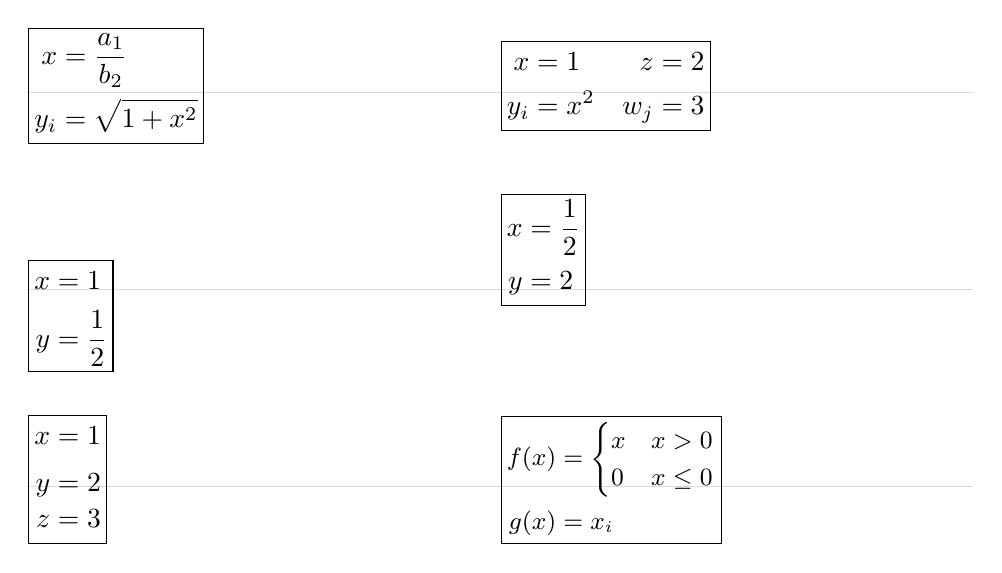
\begin{tikzpicture}
  \draw[gray!30] (0,0)--(12,0) (0,-2.5)--(12,-2.5) (0,-5)--(12,-5);
  \node[anchor=base west,draw,inner sep=2pt] at (0,0) {$\begin{aligned}x&=\frac{a_1}{b_2}\\y_i&=\sqrt{1+x^2}\end{aligned}$};
  \node[anchor=base west,draw,inner sep=2pt] at (6,0) {$\begin{aligned}x&=1&z&=2\\y_i&=x^2&w_j&=3\end{aligned}$};
  \node[anchor=base west,draw,inner sep=2pt] at (0,-2.5) {$\begin{aligned}[t]x&=1\\y&=\frac{1}{2}\end{aligned}$};
  \node[anchor=base west,draw,inner sep=2pt] at (6,-2.5) {$\begin{aligned}[b]x&=\frac{1}{2}\\y&=2\end{aligned}$};
  \node[anchor=base west,draw,inner sep=2pt] at (0,-5) {$\begin{aligned}x&=1\\[2pt]y&=2\\[-2pt]z&=3\end{aligned}$};
  \node[anchor=base west,draw,inner sep=2pt,font=\small] at (6,-5) {$\begin{aligned}f(x)&=\begin{cases}x&x>0\\0&x\leq0\end{cases}\\g(x)&=x_i\end{aligned}$};
\end{tikzpicture}
\end{document}
